\documentclass[11pt,letterpaper]{article}
\usepackage[lmargin=1in,rmargin=1in,tmargin=1in,bmargin=1in]{geometry}
\usepackage{../style/homework}
\usepackage{../style/commands}
\setbool{quotetype}{false} % True: Side; False: Under
\setbool{hideans}{false} % Student: True; Instructor: False

% -------------------
% Content
% -------------------
\begin{document}

\homework{4: Due 05/31}{Nothing has such power to broaden the mind as the ability to investigate systematically and truly all that comes under thy observation in life.}{Marcus Aurelius}

% Problem 1
\problem{10} Determine if the relations $f(x)$ and $g(x)$ shown below are functions. Explain why or why not. If the relation is a function, determine its domain, codomain, and range. 
	\[
	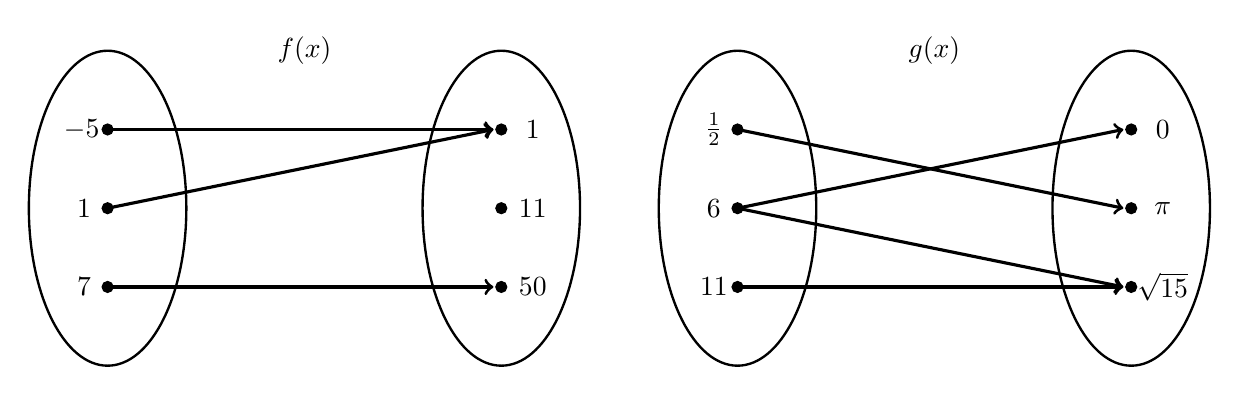
\begin{tikzpicture}
	\node at (2.5,2) {$f(x)$};
	% Ellipses
	\draw[line width=0.03cm] (0,0) circle (1 and 2);
	\draw[line width=0.03cm] (5,0) circle (1 and 2);
	
	% Nodes
	\draw[fill=black] (0,1) circle (0.07);
	\draw[fill=black] (0,0) circle (0.07);
	\draw[fill=black] (0,-1) circle (0.07);
	
	\draw[fill=black] (5,1) circle (0.07);
	\draw[fill=black] (5,0) circle (0.07);
	\draw[fill=black] (5,-1) circle (0.07);
	
	% Arrow
	\draw[line width=0.04cm,->] (0,1) -- (4.9,1);
	\draw[line width=0.04cm,->] (0,0) -- (4.9,1);
	\draw[line width=0.04cm,->] (0,-1) -- (4.9,-1);
	
	% Labels
	\node at (-0.3,1) {$\!-5$};
	\node at (-0.3,0) {$1$};
	\node at (-0.3,-1) {$7$};
	
	\node at (5.4,1) {$1$};
	\node at (5.4,0) {$11$};
	\node at (5.4,-1) {$50$};
	
	\tikzset{shift={(8,0)}}
	%
	\node at (2.5,2) {$g(x)$};
	% Ellipses
	\draw[line width=0.03cm] (0,0) circle (1 and 2);
	\draw[line width=0.03cm] (5,0) circle (1 and 2);
	
	% Nodes
	\draw[fill=black] (0,1) circle (0.07);
	\draw[fill=black] (0,0) circle (0.07);
	\draw[fill=black] (0,-1) circle (0.07);
	
	\draw[fill=black] (5,1) circle (0.07);
	\draw[fill=black] (5,0) circle (0.07);
	\draw[fill=black] (5,-1) circle (0.07);
	
	% Arrow
	\draw[line width=0.04cm,->] (0,1) -- (4.9,0);
	\draw[line width=0.04cm,->] (0,0) -- (4.9,1);
	\draw[line width=0.04cm,->] (0,0) -- (4.9,-1);
	\draw[line width=0.04cm,->] (0,-1) -- (4.9,-1);
	
	% Labels
	\node at (-0.3,1) {$\frac{1}{2}$};
	\node at (-0.3,0) {$6$};
	\node at (-0.3,-1) {$11$};
	
	\node at (5.4,1) {$0$};
	\node at (5.4,0) {$\pi$};
	\node at (5.4,-1) {$\sqrt{15}$};
	\end{tikzpicture}
	\] \pspace

\sol The relation $f(x)$ is a function because for each input there is a single possible output. We can see $f(-5)= 1$, $f(1)= 1$, and $f(7)= 50$. We can easily identify the domain, codomain, and range of $f(x)$:
	\[
	\begin{aligned}
	\text{Domain } f(x)&= \{ -5, 1, 7 \} \\
	\text{Codomain } f(x)&= \{ 1, 11, 50 \} \\
	\text{Range } f(x)&= \{ 1, 50 \}
	\end{aligned}
	\]
The relation $g(x)$ is not a function because there are inputs which have more than one possible output, i.e. there are values that are not well defined. Specifically, we see that $g(6)$ is not well defined. Therefore, $g(x)$ is not a function. 



\newpage



% Problem 2
\problem{10} Determine if the relations $f(x)$ and $g(x)$ shown below are functions. Explain why or why not. If the relation is a function, compute the functions value at $x= 4$. 
	\[
	\begin{aligned}
	f(x)&= 67.3 - 9.7x \\[0.3cm]
	g(x)&= 11.1x^2 - 15.7x + 12.9
	\end{aligned}
	\] \pspace

\sol Both $f(x)$ and $g(x)$ are functions because for each input there is a single possible output---namely, the one obtained by `evaluation' at a particular value of $x$. We can easily evaluate each function at $x= 4$: \pspace
	\[
	\begin{aligned}
	f(4)&= 67.3 - 9.7(4)=  67.3 - 38.8= 28.5 \\[0.3cm]
	g(4)&= 11.1(4^2) - 15.7(4) + 12.9= 177.6 - 62.8 + 12.9= 127.7
	\end{aligned}
	\]



\newpage



% Problem 3
\problem{10} Suppose $f(x)$ and $g(x)$ are the functions given below. 
        \begin{table}[!ht]
        \centering
        \begin{tabular}{| c || r | r | r | r | r | r | r |} \hline
	$x$ & $-3$ & $-2$ & $-1$ & $\phantom{-}0$ & $\phantom{-}1$ & $\phantom{-}2$ & $\phantom{-}3$ \\ \hline
	$f(x)$ & $6$ & $0$ & $-4$ & $5$ & $4$ & $-3$ & $2$ \\ \hline
	$g(x)$ & $0$ & $3$ & $1$ & $1$ & $2$ & $9$ & $6$ \\ \hline
	$h(x)$ & $-1$ & $5$ & $-8$ & $-3$ & $8$ & $2$ & $0$ \\ \hline
        \end{tabular}
        \end{table}

Compute the following: \pspace
        \begin{enumerate}[(a)]
        \item $(g + h)(1)= g(1) + h(1)= 2 + 8= 10$ \vfill
        \item $(g - f)(0)= g(0) - f(0)= 1 - 5= -4$ \vfill
        \item $(-2h)(3)= -2h(3)= -2(0)= 0$ \vfill
        \item $\left(\dfrac{h}{g}\right)(2)= \dfrac{h(2)}{g(2)}= \dfrac{2}{9}$ \vfill
        \item $f(1)\, h(-1)= 4 \cdot -8= -32$ \vfill
        \item $f(-1 - h(0))= f(-1 - -3)= f(2)= -3$ \vfill
        \item $(f \circ g)(-2)= f(g(-2))= f(3)= 2$ \vfill
	\item $(g \circ h)(-3)= g(h(-3))= g(-1)= 1$ \vfill
        \item $(h \circ g)(-3)= h(g(-3))= h(0)= -3$ \vfill
	\item $(h \circ f \circ g)(1)= h(f(g(1))= h(f(2))= h(-3)= -1$ \vfill
        \end{enumerate} 



\newpage



% Problem 4
\problem{10} Suppose $f(x)$ and $g(x)$ are the functions given below. 
	\[
	\begin{aligned}
	f(x)&= 5x - 6 \\[0.3cm]
	g(x)&= 3x + 1
	\end{aligned}
	\]

Compute the following: \pspace
        \begin{enumerate}[(a)]
        \item $g(2)= 3(2) + 1= 6 + 1= 7$ \vfill
        \item $f(-1)= 5(-1) - 6= -5 - 6= -11$ \vfill
        \item $2f(1) - g(2)= 2 \big( 5(1) - 6 \big) - \big( 3(2) + 1 \big)= 2(5 - 6) - (6 + 1)= 2(-1) - 7= -2 - 7= -9$ \vfill
        \item $f(x) - g(x)= (5x - 6) - (3x + 1)= 5x - 6 - 3x - 1= 2x - 7$ \vfill
        \item $f(x) \, g(x)= (5x - 6)(3x + 1)= 15x^2 + 5x - 18x - 6= 15x^2 - 13x - 6$ \vfill
        \item $\left( \dfrac{f}{g} \right)(x)= \dfrac{5x - 6}{3x + 1}$ \vfill
        \item $(f \circ g)(0)= f(g(0))= f\big( 3(0) + 1 \big)= f(0 + 1)= f(1)= 5(1) - 6= 5 - 6= -1$ \vfill
        \item $(g \circ f)(1)= g(f(1))= g\big( 5(1) - 6 \big)= g(5 - 6)= g(-1)= 3(-1) + 1= -3 + 1= -2$ \vfill
        \item $(f \circ g)(x)= f(g(x))= f(3x + 1)= 5(3x + 1) - 6= 15x + 5 - 6= 15x - 1$ \vfill
        \item $(g \circ f)(x)= g(f(x))= g(5x - 6)= 3(5x - 6) + 1= 15x - 18 + 1= 15x - 17$ \vfill
        \end{enumerate} 



\newpage



% Problem 5
\problem{10} Determine if the relation below is a function or not. If it is a function, explain why. If it is not a function, explain why. 
	\[
	\fbox{
	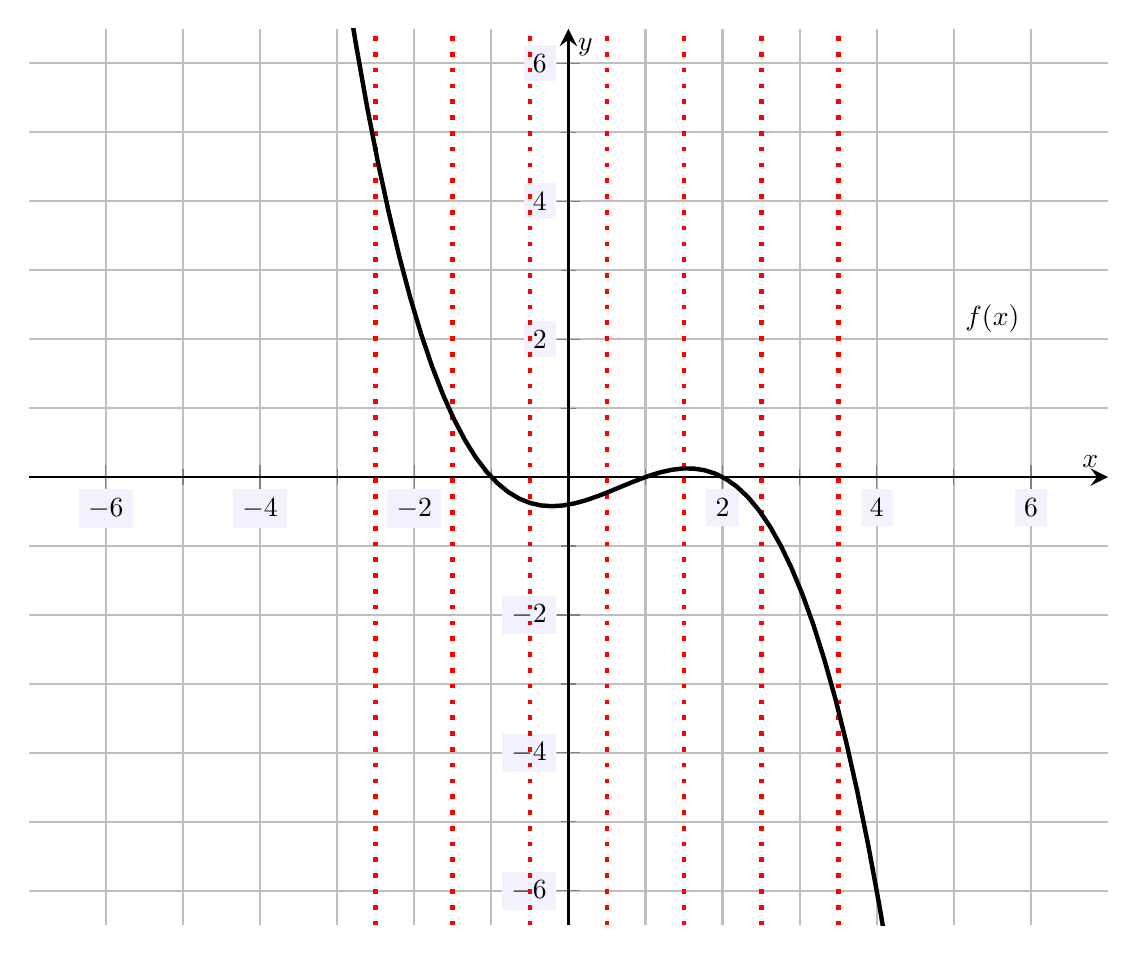
\begin{tikzpicture}[scale=2,every node/.style={scale=0.5}]
	\begin{axis}[
	grid=both,
	axis lines=middle,
	ticklabel style={fill=blue!5!white},
	xmin= -7, xmax=7,
	ymin= -6.5, ymax=6.5,
	xtick={-6,-4,-2,0,2,4,6},
	ytick={-6,-4,-2,0,2,4,6},
	minor tick = {-5,-3,...,5},
	xlabel=\(x\),ylabel=\(y\),
	]
	\pgfplotsinvokeforeach {-2.5,-1.5,...,3.5} {
		\draw[red,dotted,line width= 0.03cm] (#1, -6.5) -- (#1, 6.5);
	}
	\node at (5.5,2.3) {$f(x)$};
	\addplot[thick, domain= -7:7, samples=100] ({x},{-1/5*(x + 1)*(x - 2)*(x -1)});
	\end{axis}
	\end{tikzpicture}
	}
	\] \pspace

\sol The relation in the graph above is a function because it passes the vertical line test, i.e. every vertical line intersects the function at most once.



\newpage



% Problem 6
\problem{10} Determine whether the point $(3, -4)$ is on the graph of $f(x)= \dfrac{x + 1}{x - 4}$. Determine also whether the point $(9, -2)$ is on the graph of $f(x)$. For each, explain why or why not. \pspace

\sol We know that $f(x)= \dfrac{x + 1}{x - 4}$ is a function because for each input there is only a single possible output---namely, the one obtained by evaluation. We have\dots 
	\[
	f(3)= \dfrac{3 + 1}{3 - 4}= \dfrac{4}{-1}= -4.
	\]
This implies that the point $(3, -4)$ is a point on the graph of $f(x)$. However, we have\dots
	\[
	f(9)= \dfrac{9 + 1}{9 - 4}= \dfrac{10}{5}= 2
	\]
so that $(9, 2)$ is a point on the graph. But then because $f(x)$ is a function, $(9, -2)$ cannot be a point on the graph of $f(x)$. 



\newpage



% Problem 7
\problem{10} On the plot below and as accurately as possible, sketch the function $f(x)= \dfrac{2x^2 - 5}{x + 11}$. 
	\[
	\fbox{
	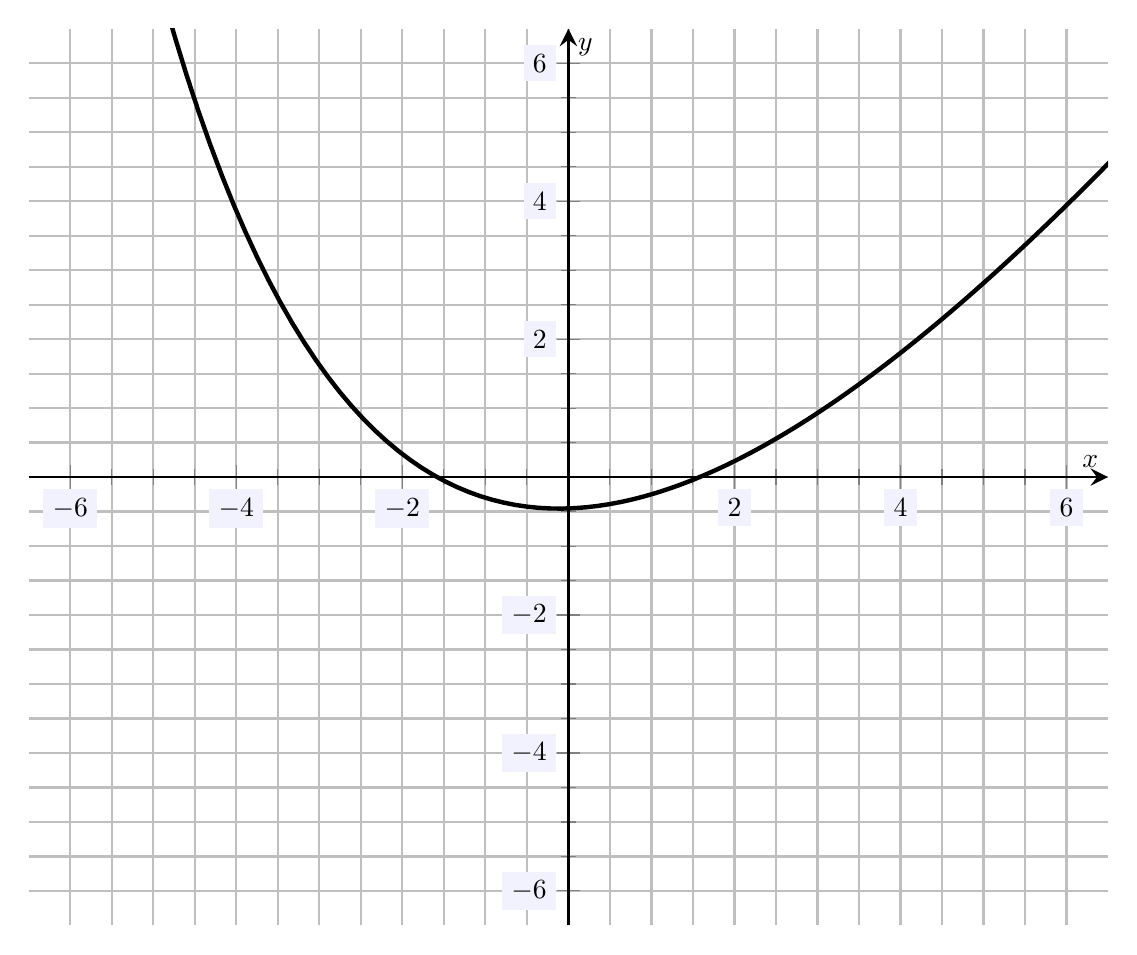
\begin{tikzpicture}[scale=2,every node/.style={scale=0.5}]
	\begin{axis}[
	grid=both,
	axis lines=middle,
	ticklabel style={fill=blue!5!white},
	xmin= -6.5, xmax=6.5,
	ymin= -6.5, ymax=6.5,
	xtick={-6,-4,-2,0,2,4,6},
	ytick={-6,-4,-2,0,2,4,6},
	minor tick = {-6,-5.5,-5,...,6},
	xlabel=\(x\),ylabel=\(y\),
	]
	\addplot[thick, domain= -7:7, samples=100] ({x},{(2*x^2 - 5)/(x + 11)});
	\end{axis}
	\end{tikzpicture}
	}
	\] \pspace

\sol To plot the function $f(x)= \dfrac{2x^2 - 5}{x + 11}$, we create a table of values for $f(x)$ and plot these points, connecting them up as smoothly as possible. For instance, we have\dots
	\[
	f(3)= \dfrac{2(3^2) - 5}{3 + 11}= \dfrac{2(9) - 5}{14}= \dfrac{18 - 5}{14}= \dfrac{13}{14} \approx 0.928571.
	\]
We have\dots
	\begin{table}[!ht]
	\centering
	\begin{tabular}{c||r|r|r|r|r|r|r|r|r|r|r|r|r}
	$x$ & $-6$ & $-5$ & $-4$ & $-3$ & $-2$ & $1$ & $0$ & $1$ & $2$ & $3$ & $4$ & $5$ & $6$ \\ \hline
	$f(x)$ & $\tfrac{67}{5}$ & $\tfrac{15}{2}$ & $\tfrac{27}{7}$ & $\tfrac{13}{8}$ & $\tfrac{1}{3}$ & $-\tfrac{3}{10}$ & $-\tfrac{5}{11}$ & $-\tfrac{1}{4}$ & $\tfrac{3}{13}$ & $\tfrac{13}{14}$ & $\tfrac{9}{5}$ & $\tfrac{45}{16}$ & $\tfrac{67}{17}$
	\end{tabular}
	\end{table}
or approximate values\dots
	\begin{table}[!ht]
	\centering
	\begin{tabular}{c||r|r|r|r|r|r|r|r|r|r|r|r|r}
	$x$ & $-6$ & $-5$ & $-4$ & $-3$ & $-2$ & $1$ & $0$ & $1$ & $2$ & $3$ & $4$ & $5$ & $6$ \\ \hline
	$f(x)$ & $13.4$ & $7.5$ & $3.9$ & $1.6$ & $0.3$ & $-0.3$ & $-0.5$ & $-0.3$ & $0.2$ & $0.9$ & $1.8$ & $2.8$ & $3.9$
	\end{tabular}
	\end{table}



\newpage



% Problem 8
\problem{10} Explain why the function sketched below has an inverse and then sketch its inverse. 
	\[
	\fbox{
	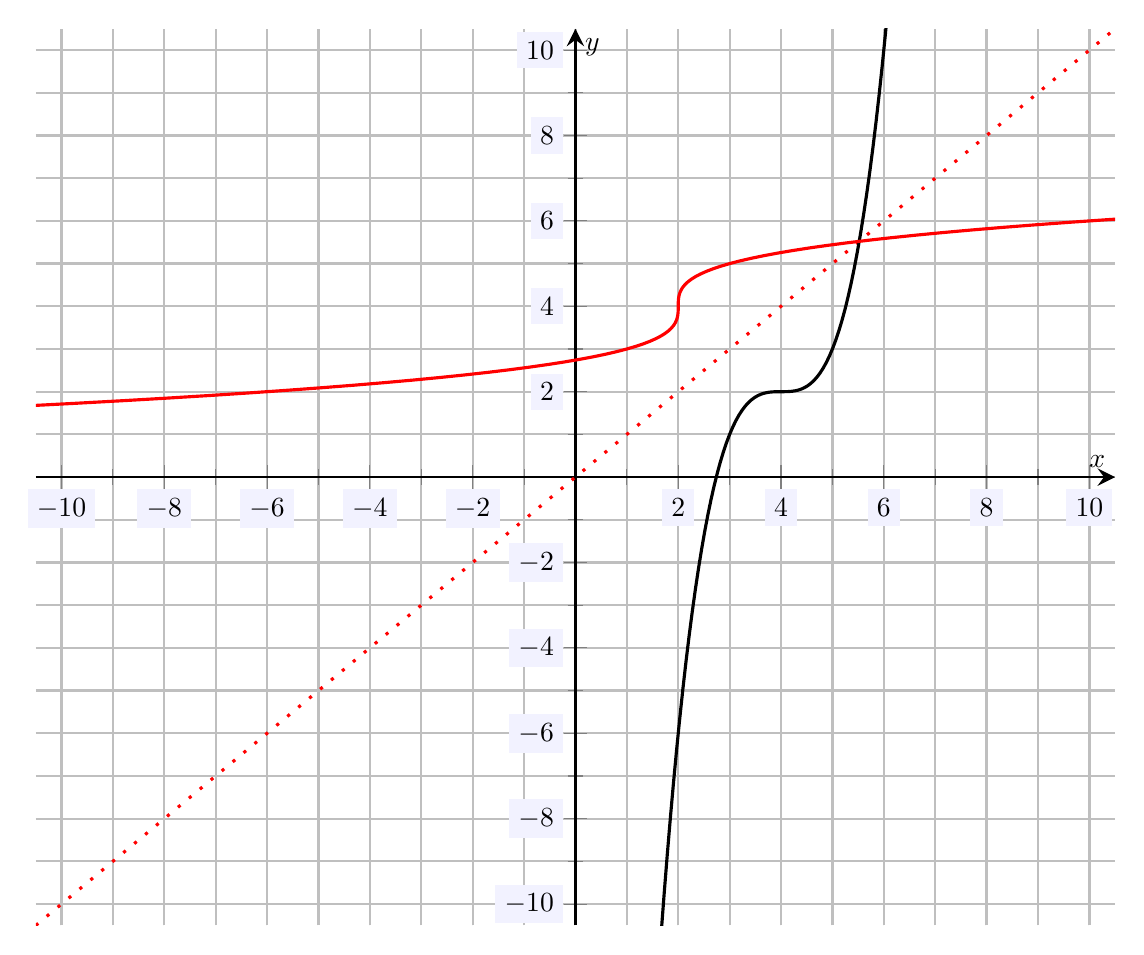
\begin{tikzpicture}[scale=2,every node/.style={scale=0.5}]
	\begin{axis}[
	grid=both,
	axis lines=middle,
	ticklabel style={fill=blue!5!white},
	xmin= -10.5, xmax=10.5,
	ymin= -10.5, ymax=10.5,
	xtick={-10,-8,-6,-4,-2,0,2,4,6,8,10},
	ytick={-10,-8,-6,-4,-2,0,2,4,6,8,10},
	minor tick = {-10,-9,...,10},
	xlabel=\(x\),ylabel=\(y\),
	]
	\addplot[red,dotted,line width= 0.02cm,domain= -10.5:10.5] ({x},{x}); 
	\addplot[line width= 0.02cm,domain= 1:7,samples=100] ({x},{(x - 4)^3 + 2}); 
	\addplot[red,line width= 0.02cm,domain= 1:7,samples=100] ({(x - 4)^3 + 2},{x}); 
	\end{axis}
	\end{tikzpicture}
	}
	\] \pspace

\sol The function above has an inverse because it passes the horizontal line test, i.e. every horizontal line intersects the function at most once. To sketch the inverse, we reflect the graph of the function through the line $y= x$ (the dotted line in the plot above), which yields the red curve above.  



\newpage



% Problem 9
\problem{10} How many $y$-intercepts can a function have? Explain. Is this the same for $x$-intercepts? Explain. \pspace

\sol A function can have at most one $y$-intercept. If a function had more than one $y$-intercept, then the function would not be well defined at $x= 0$, i.e. it would fail the vertical line test. It is possible for a function to have no $y$-intercept, e.g. $f(x)= \frac{1}{x}$. On the other hand, a function can have any amount of $x$-intercepts. For instance, $f(x)= 1$ has no $x$-intercepts as it is parallel to the $x$-axis. The function $f(x)= x$ has one $x$-intercept, while the function $f(x)= x(x - 1)$ has two $y$-intercepts. Furthermore, the function $f(x)= x(x - 1)(x - 2) \cdots (x - n)$ has $n + 1$ $x$-intercepts. The function $f(x)= \sin x$ has infinitely many $x$-intercepts. 



\newpage



% Problem 10
\problem{10} Using the concept of range and the fact that every non-horizontal line $\ell(x)$ intersects any horizontal line, explain why the equation $\ell(x)= c$ has a solution for every real number $c$. \pspace

\sol Suppose that $\ell(x)$ is a non-horizontal line. Then given the horizontal line $y= c$, we know that $\ell(x)$ will intersect the line $y= c$, suppose at $(x_0, c)$. This means that the range of $\ell(x)$ is all real numbers. But then there is an $x$, namely $x_0$, such that $\ell(x_0)= c$. Therefore, the equation $\ell(x)= c$ has a solution. 


\end{document}